\documentclass{article}
\usepackage{graphicx}
\usepackage[margin=1.5cm]{geometry}
\usepackage{amsmath}

\begin{document}

\title{Monday Reading Assessment: Unit 2, Ohm's Law and Batteries, Kirchhoff's Rules}
\author{Prof. Jordan C. Hanson}

\maketitle

\section{Memory Bank}

\begin{itemize}
\item $V = IR$ ... Ohm's Law
\item $R^{-1}_{\rm tot} = R_1^{-1} + R_2^{-1} + ...$ ... Adding resistors in parallel.
\item $R_{\rm tot} = R_1 + R_2 + ...$ ... Adding resistors in series.
\item $P = IV$ ... Power in DC circuits
\end{itemize}

\section{Complex Circuit}

\begin{enumerate}
\item (a) What is the total resistance in Fig. \ref{fig:dura}? (b) Find the current supplied by the source $V$. (c) Calculate the currents in each resistor and show that these add together to equal the current output of the source. (d) Calculate the power dissipated by each resistor. (e) Find the power output of the source and show that it equals the total power dissipated by the resistors.
\begin{figure}[ht]
\centering
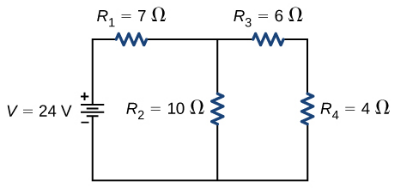
\includegraphics[width=0.5\textwidth]{circuit_series_parallel.png}
\caption{\label{fig:dura} A circuit involving four resistors.}
\end{figure}
\end{enumerate}

\end{document}
